

\tikzset{every picture/.style={line width=0.75pt}} %set default line width to 0.75pt        

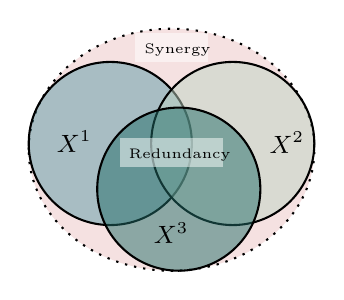
\begin{tikzpicture}[x=0.75pt,y=0.75pt,yscale=-1,xscale=1]
%uncomment if require: \path (0,300); %set diagram left start at 0, and has height of 300

%Shape: Ellipse [id:dp7373298723691162] 
\draw  [fill={rgb, 255:red, 206; green, 106; blue, 107 }  ,fill opacity=0.2 ][dash pattern={on 0.84pt off 2.51pt}] (71.4,159.3) .. controls (71.4,127.1) and (102.2,101) .. (140.2,101) .. controls (178.2,101) and (209,127.1) .. (209,159.3) .. controls (209,191.5) and (178.2,217.6) .. (140.2,217.6) .. controls (102.2,217.6) and (71.4,191.5) .. (71.4,159.3) -- cycle ;
%Shape: Circle [id:dp03598595550859773] 
\draw  [fill={rgb, 255:red, 74; green, 145; blue, 158 }  ,fill opacity=0.45 ] (71.4,156.3) .. controls (71.4,134.6) and (89,117) .. (110.7,117) .. controls (132.4,117) and (150,134.6) .. (150,156.3) .. controls (150,178) and (132.4,195.6) .. (110.7,195.6) .. controls (89,195.6) and (71.4,178) .. (71.4,156.3) -- cycle ;
%Shape: Circle [id:dp05882206005366952] 
\draw  [fill={rgb, 255:red, 190; green, 211; blue, 195 }  ,fill opacity=0.5 ] (130.4,156.3) .. controls (130.4,134.6) and (148,117) .. (169.7,117) .. controls (191.4,117) and (209,134.6) .. (209,156.3) .. controls (209,178) and (191.4,195.6) .. (169.7,195.6) .. controls (148,195.6) and (130.4,178) .. (130.4,156.3) -- cycle ;
%Shape: Circle [id:dp6392767984689582] 
\draw  [fill={rgb, 255:red, 34; green, 109; blue, 104 }  ,fill opacity=0.5 ] (104.4,178.3) .. controls (104.4,156.6) and (122,139) .. (143.7,139) .. controls (165.4,139) and (183,156.6) .. (183,178.3) .. controls (183,200) and (165.4,217.6) .. (143.7,217.6) .. controls (122,217.6) and (104.4,200) .. (104.4,178.3) -- cycle ;

% Text Node
\draw (83.45,148.97) node [anchor=north west][inner sep=0.75pt]  [font=\small,rotate=-359.65]  {$X^{1}$};
% Text Node
\draw (130.16,192.97) node [anchor=north west][inner sep=0.75pt]  [font=\small,rotate=-359.65]  {$X^{3}$};
% Text Node
\draw (185.9,149.47) node [anchor=north west][inner sep=0.75pt]  [font=\small,rotate=-359.65]  {$X^{2}$};
% Text Node
\draw  [draw opacity=0][fill={rgb, 255:red, 255; green, 255; blue, 255 }  ,fill opacity=0.5 ]  (122.7,103) -- (157.7,103) -- (157.7,117) -- (122.7,117) -- cycle  ;
\draw (125.7,107) node [anchor=north west][inner sep=0.75pt]  [font=\tiny,color={rgb, 255:red, 0; green, 0; blue, 0 }  ,opacity=1 ] [align=left] {Synergy};
% Text Node
\draw  [draw opacity=0][fill={rgb, 255:red, 255; green, 255; blue, 255 }  ,fill opacity=0.5 ]  (115.2,153.5) -- (165.2,153.5) -- (165.2,167.5) -- (115.2,167.5) -- cycle  ;
\draw (118.2,157.5) node [anchor=north west][inner sep=0.75pt]  [font=\tiny,color={rgb, 255:red, 0; green, 0; blue, 0 }  ,opacity=1 ] [align=left] {Redundancy};


\end{tikzpicture}
